\chapter{Unit Test}
I følgende afsnit beskrives de unit test der bliver lavet. Der bruges Nunit\cite{NUnit}, som er en testing framework til vores testing af klasser. 

Diverse klasser vil blive testet i Testklassen af følgende syntaks "\big[Klasse\big]Unit". Methoderne skrevet i test klassen er skrevet med henblik over at det skal være lidt læseligt, og er opsat med følgende syntaks: 
\big[Hvad der testes\big]\_[I hvilke slags senarier]\_\big[og den forventet resultat\big] 

\section{Validator}
Validator-klassen er en statisk klasse, som har ansvar for at håndtere validering af input felterne i applikationen fra brugeren. For eksempel kan det være når brugeren skal indtaste sin email og password. På figur \ref{fig:ValidatorUnit} ses følgende test der bliver udført.
\begin{figure}[H]
	\centering
	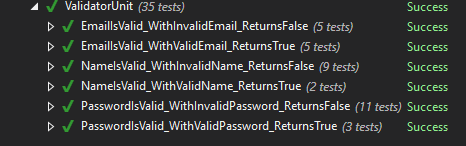
\includegraphics[width=0.6\linewidth]{Unit/ValidatorUnit.PNG}
	\caption{Her ses et screenshot af test sessionen på ValidatorUnit}
	\label{fig:ValidatorUnit}
\end{figure}
 Der testes kun for Validator klassen fordi at det er den eneste klasse, der har noget algorithme. Da meget af koden som der benyttes ligger i forskelllige frameworks, tages der højde for at disse er vel implementeret og gennemtestet, så derfor er der ikke implementeret mere test. 
\clearpage

På Figur \ref{fig:ValidatorUnitEmail} ses følgende test på e-mail der bliver udført. Her ses hvilket format af e-mail vi tillader for at sikre klassen fungerer som ønsket.
Der bliver udført både negativ og positiv test på e-mails, for at tjekke at både de ønskede og uønskede værdier bliver godkendt. Funktionen EmailIsValid tjekker at E-mail opfylder bland andet disse krav:\\
\begin{itemize}
	\item E-mail må ikke have mellemskarakter
	\item Domæne navnet må ikke være tomt
	\item Top level domain navnet\cite{TLD} må ikke være tomt
	\item Lokal navn må ikke være tomt
	\item Lokal navn må ikke starte eller slutte med et punktum
	\item Lokal navn må ikke være tomt
	\item Lokal navn må ikke starte eller slutte med et punktum
	
\end{itemize}

\begin{figure}[H]
	\centering
	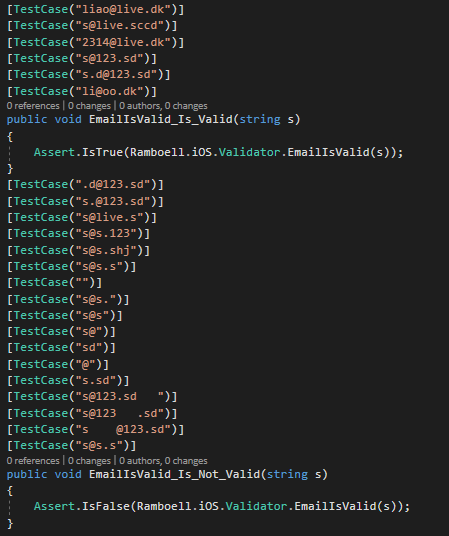
\includegraphics[width=0.6\linewidth]{Unit/ValidatorUnitEmail.PNG}
	\caption{Her ses et screenshot af test sessionen på ValidatorUnit e-mail}
	\label{fig:ValidatorUnitEmail}
\end{figure}

\clearpage

På Figur \ref{fig:ValidatorUnitPassword} ses både positive og negative tests på funktionen PasswordIsValid. Der bliver givet et password som funktion vil godkende og et password som ikke bliver godkendt. Der bliver også tjekket op mod at der bliver givet det forventet resultat. Funktionen PasswordIsValid tjekker at et password opfylder disse krav: \\
\begin{itemize}
	\item Minimum 6 karakter lang
	\item Minimum et stort bogstav
	\item Minimum et lille bogstav
	\item Minimum et tal
	\item Speciel tegn er valgfrit
	\item Må ikke have mellemrum
\end{itemize}

\begin{figure}[H]
	\centering
	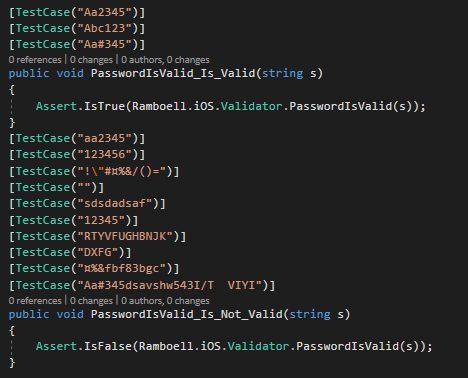
\includegraphics[width=0.6\linewidth]{Unit/ValidatorUnitPassword.PNG}
	\caption{Her ses et screenshot af test sessionen på ValidatorUnit på password}
	\label{fig:ValidatorUnitPassword}
\end{figure}

Der testes kun for Validator klassen fordi at det er den eneste klasse, der har noget algorithme. Da meget af koden som der benyttes ligger i forskelllige frameworks, tages der højde for at disse er vel implementeret og gennemtestet, så derfor, er der ikke implementeret flere test. 

